% !TEX TS-program = pdflatex
% !TEX encoding = UTF-8 Unicode

\documentclass[12pt, a4paper]{article}
\usepackage[utf8]{inputenc}
\usepackage[T1]{fontenc}
\usepackage{helvet}
\usepackage{graphicx}
\usepackage{geometry}
\usepackage{rotating}
\geometry{a4paper, landscape, margin=1.5cm}
\renewcommand{\familydefault}{\sfdefault}
\pagestyle{empty}

\begin{document}

% Top half (upside down, at the top)
\vspace*{0pt}
\begin{center}
  \begin{rotate}{180}
    \begin{minipage}[c][0.45\textheight][c]{0.95\textwidth}
      \begin{minipage}[c]{0.45\textwidth}
        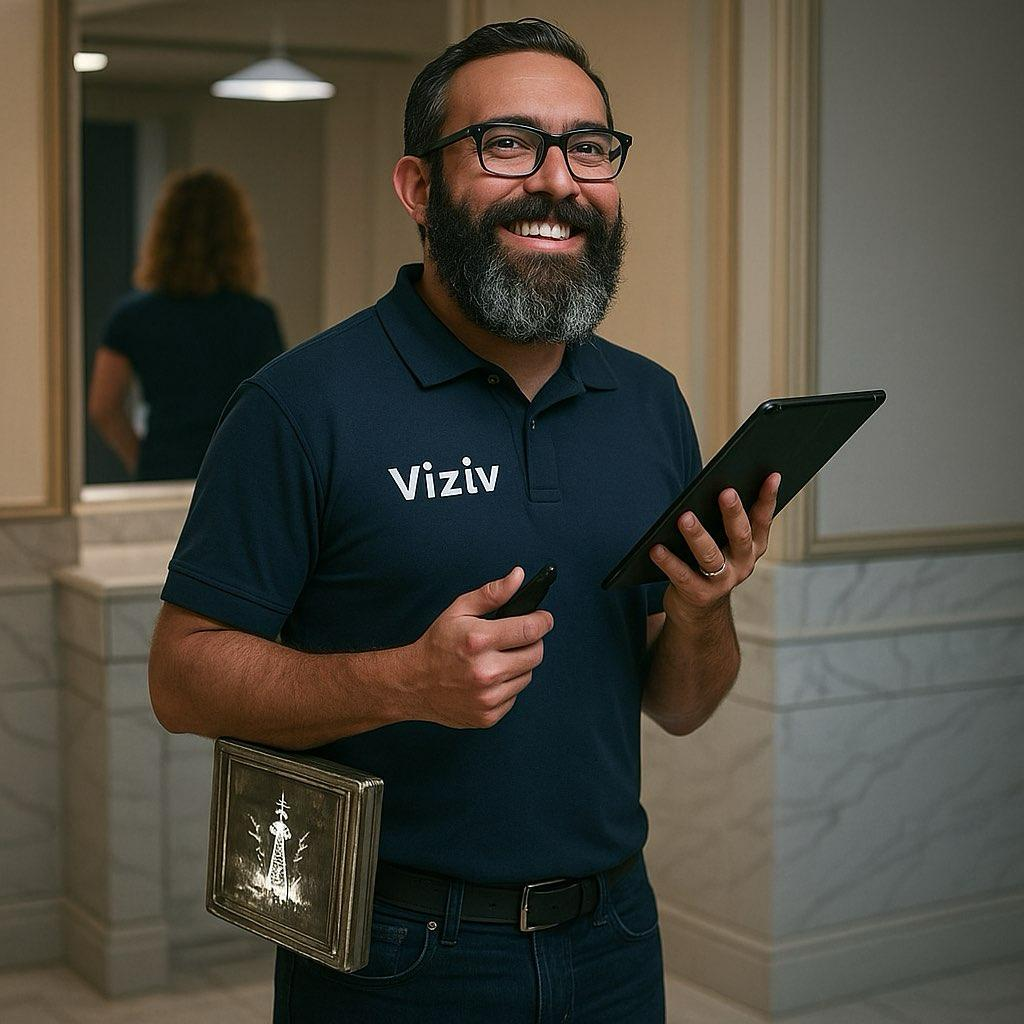
\includegraphics[height=7cm,keepaspectratio]{Karl.jpeg}
      \end{minipage}%
      \begin{minipage}[c]{0.54\textwidth}
        \centering
        {\fontsize{40}{48}\selectfont Field Technician Karl} \\[1cm]
        {\Large\itshape "If duct tape can't fix it, you didn't use enough duct tape."}
      \end{minipage}
    \end{minipage}
  \end{rotate}
\end{center}

% Space between halves
\vspace*{0.1\textheight}

% Bottom half (right side up, at the bottom)
\begin{center}
  \begin{minipage}[c][0.45\textheight][c]{0.95\textwidth}
    \begin{minipage}[c]{0.45\textwidth}
      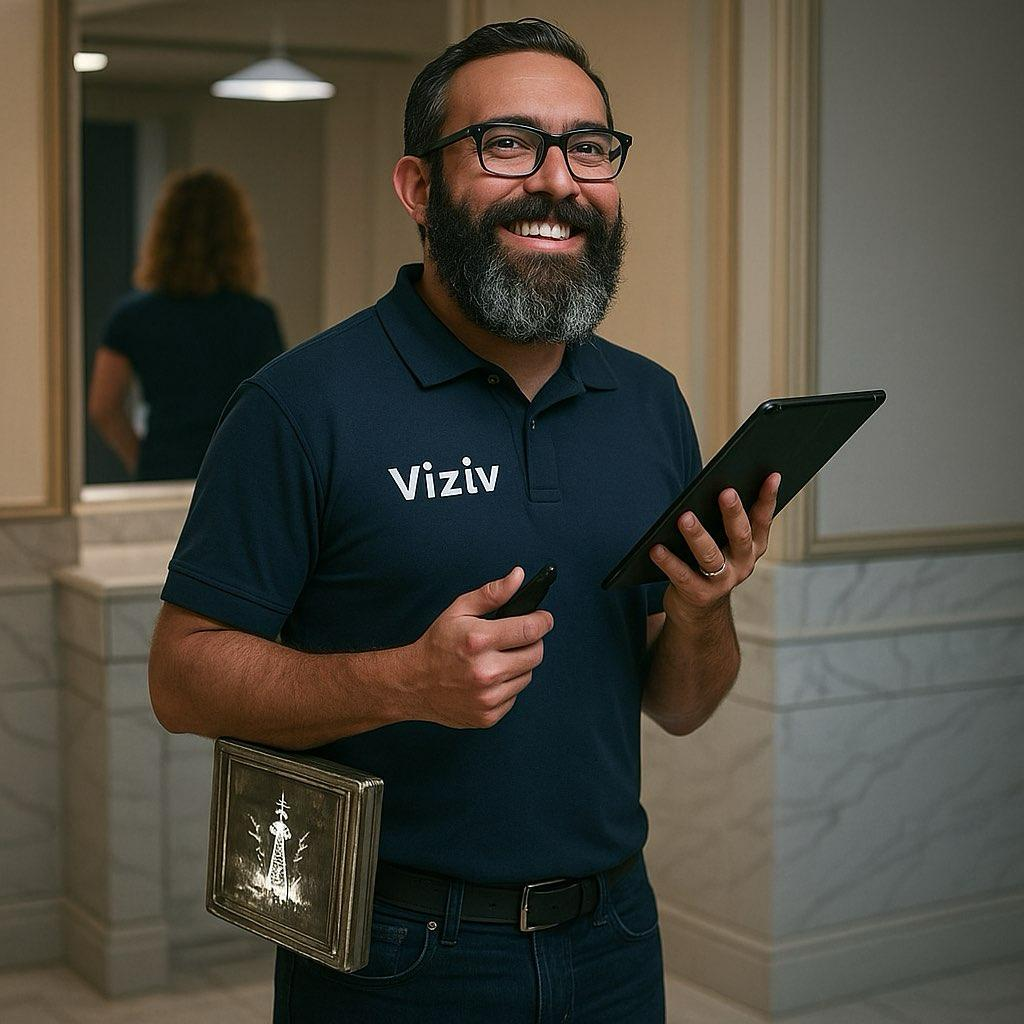
\includegraphics[height=7cm,keepaspectratio]{Karl.jpeg}
    \end{minipage}%
    \begin{minipage}[c]{0.54\textwidth}
      \centering
      {\fontsize{40}{48}\selectfont Field Technician Karl} \\[1cm]
      {\Large\itshape "If duct tape can't fix it, you didn't use enough duct tape."}
    \end{minipage}
  \end{minipage}
\end{center}

\end{document} 